\documentclass[11pt]{article}
\usepackage[a4paper,margin=2.3cm]{geometry}
\usepackage{amsmath,amssymb,booktabs,xcolor,tikz,caption,subcaption}
\usepackage{hyperref}
\usepackage{cleveref}
\usetikzlibrary{arrows.meta,positioning,shapes.geometric,calc}

\newcommand{\F}{\mathbb{F}_2}
\newcommand{\rowsp}{\operatorname{row}}
\newcommand{\rk}{\operatorname{rank}}

% ---------------------------------------------------------------- colours
\definecolor{Lc}{HTML}{0072B2}   % L qubits
\definecolor{Rc}{HTML}{D55E00}   % R qubits
\definecolor{Xc}{HTML}{CC3311}   % X checks
\definecolor{Zc}{HTML}{009E73}   % Z checks
\definecolor{faint}{HTML}{C8C8C8}

% Layout = the toric-code lattice, x to the right, y up. X checks on vertices, Z checks on
% faces, L qubits on vertical edges, R qubits on horizontal edges. Each block is drawn with a
% fixed offset so that the local legs of every check (y, y^2 on L; x, x^2 on R) are its four
% nearest edges:
%   L(a,b) at (a, b)              X(a,b) at (a, b+1.5)
%   R(a,b) at (a-1.5, b+1.5)      Z(a,b) at (a-1.5, b)
\tikzset{
  Lq/.style={circle, fill=Lc, inner sep=0pt, minimum size=5pt},
  Rq/.style={circle, fill=Rc, inner sep=0pt, minimum size=5pt},
  Xck/.style={rectangle, fill=Xc, inner sep=0pt, minimum size=5pt},
  Zck/.style={rectangle, fill=Zc, inner sep=0pt, minimum size=5pt},
  dot/.style={circle, fill=faint, inner sep=0pt, minimum size=1.6pt},
  origin/.style={circle, draw=black, thick, inner sep=0pt, minimum size=9pt},
  link/.style={-{Stealth[length=4pt]}, thick},
  lat/.style={faint!70, very thin},
}
% unwrapped positions (local windows; arguments may be negative)
\newcommand{\Lpos}[2]{({#1}, {#2})}
\newcommand{\Xpos}[2]{({#1}, {#2+1.5})}
\newcommand{\Rpos}[2]{({#1-1.5}, {#2+1.5})}
\newcommand{\Zpos}[2]{({#1-1.5}, {#2})}
% wrapped positions on the torus (a in 0..5, b in 0..11), inside [-0.25,5.75] x [-0.25,11.75]
\newcommand{\LposT}[2]{({#1}, {#2})}
\newcommand{\XposT}[2]{({#1}, {mod(#2+1,12)+0.5})}
\newcommand{\RposT}[2]{({mod(#1+4,6)+0.5}, {mod(#2+1,12)+0.5})}
\newcommand{\ZposT}[2]{({mod(#1+4,6)+0.5}, {#2})}
% faint lattice over a window: vertical lines at integer x, horizontal at half-integer y
\newcommand{\latwin}[4]{% x0, x1, y0, y1 (integers)
  \foreach \xx in {#1,...,#2} \draw[lat] (\xx,#3-0.3) -- (\xx,#4+0.3);
  \foreach \yy in {#3,...,#4} \draw[lat] (#1-0.3,\yy+0.5) -- (#2+0.3,\yy+0.5);}
% the whole torus, faint: lattice lines, all qubits, site (0,0) marked
\newcommand{\torus}{%
  \foreach \xx in {0,...,5} \draw[lat] (\xx,-0.25) -- (\xx,11.75);
  \foreach \yy in {0,...,11} \draw[lat] (-0.25,\yy+0.5) -- (5.75,\yy+0.5);
  \foreach \a in {0,...,5}{\foreach \b in {0,...,11}{%
    \node[dot] at \LposT{\a}{\b} {}; \node[dot] at \RposT{\a}{\b} {};}}
  \draw[faint] (-0.25,-0.25) rectangle (5.75,11.75);}

\title{Logical errors of the gross code:\\ what they are, how to find them, how to check them}
\author{rl-for-qec notes}
\date{\today}

\begin{document}
\maketitle

\noindent These notes explain the ideas behind the coset catalogue in
\texttt{src/train\_utils/coset\_catalogue.py} (exact, slow) and
\texttt{coset\_enumerate.py} (sampling, fast). Everything is linear algebra over
$\F=\{0,1\}$ (addition is XOR). We treat X-type errors; Z-type errors are the mirror image.

\tableofcontents

%======================================================================
\section{The lattice: a $6\times 12$ torus with two qubits per site}

The gross code $[[144,12,12]]$ lives on an $l\times m = 6\times 12$ grid with periodic
boundaries (a torus). A site is labelled $(a,b)$: $a\in\{0..5\}$ counts steps to the right
(the $x$ direction), $b\in\{0..11\}$ steps up (the $y$ direction).\footnote{Bravyi et al.\ write
the gross code with $l=12$, $m=6$; our configuration has $l=6$, $m=12$ with the same $A$, $B$.
Swapping $x\leftrightarrow y$ together with $L\leftrightarrow R$ maps one onto the other, so it is
the same code.} Each site carries four objects: an \textcolor{Lc}{$L$ qubit}, an
\textcolor{Rc}{$R$ qubit}, an \textcolor{Xc}{X check} and a \textcolor{Zc}{Z check}. Hence
$2\cdot 72 = 144$ data qubits, $72$ X checks and $72$ Z checks. In the code, $L$ qubit $(a,b)$
has index $12a+b$ and $R$ qubit $(a,b)$ has index $72+12a+b$.

The natural picture is the one of the toric code (\cref{fig:cell}): a square lattice with
X checks on the vertices, Z checks on the faces, $L$ qubits on the vertical edges and $R$
qubits on the horizontal edges. Drawn this way every check touches its four nearest qubits,
plus two distant ones.

\begin{figure}[h]
\centering
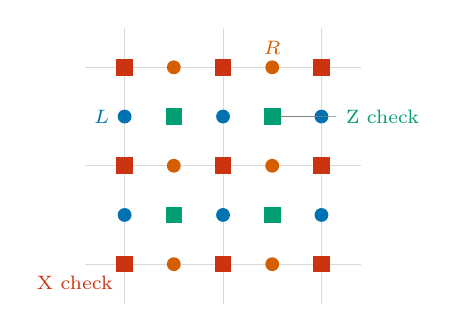
\begin{tikzpicture}[scale=1.25]
  \foreach \t in {0,1,2} {\draw[lat] (-0.4,\t) -- (2.4,\t); \draw[lat] (\t,-0.4) -- (\t,2.4);}
  \foreach \i in {0,1,2}{\foreach \j in {0,1,2}{\node[Xck, minimum size=6pt] at (\i,\j) {};}}
  \foreach \i in {0,1}{\foreach \j in {0,1}{\node[Zck, minimum size=6pt] at (\i+0.5,\j+0.5) {};}}
  \foreach \i in {0,1,2}{\foreach \j in {0,1}{\node[Lq] at (\i,\j+0.5) {};}}
  \foreach \i in {0,1}{\foreach \j in {0,1,2}{\node[Rq] at (\i+0.5,\j) {};}}
  \node[below left=1pt, font=\scriptsize, Xc] at (0,0) {X check};
  \node[Zck, minimum size=6pt, pin={[font=\scriptsize, Zc, pin distance=7mm]right:Z check}] at (1.5,1.5) {};
  \node[left=2pt, font=\scriptsize, Lc] at (0,1.5) {$L$};
  \node[above=1pt, font=\scriptsize, Rc] at (1.5,2) {$R$};
\end{tikzpicture}
\hspace{1.2cm}
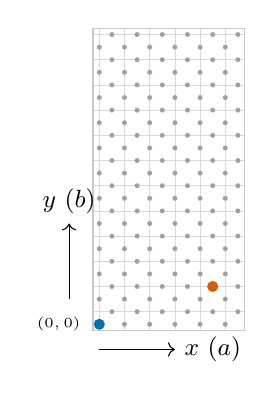
\begin{tikzpicture}[scale=0.32, dot/.style={circle, fill=faint!80!black, inner sep=0pt, minimum size=1.8pt}]
  \torus
  \node[Lq, minimum size=4pt] at \LposT{0}{0} {}; \node[Rq, minimum size=4pt] at \RposT{0}{0} {};
  \node[left=1pt, font=\tiny] at (-0.25,0) {$(0,0)$};
  \draw[->] (0,-1) -- (3,-1) node[right] {\small $x$ ($a$)};
  \draw[->] (-1.2,1) -- (-1.2,4) node[above] {\small $y$ ($b$)};
\end{tikzpicture}
\caption{Left: a patch of the lattice. X checks (red) on vertices, Z checks (green) on faces,
$L$ qubits (blue) on vertical edges, $R$ qubits (orange) on horizontal edges. Right: the whole
$6\times 12$ torus (grey dots: the 144 qubits; coloured: the $L$ and $R$ qubit of site $(0,0)$).
Leaving on one side re-enters on the other.}
\label{fig:cell}
\end{figure}

%======================================================================
\section{What does $A = x^3+y+y^2$ mean?}

\subsection{Monomials are shifts}
Let $x$ be ``move one step right'' ($a\to a+1$) and $y$ ``move one step up''
($b\to b+1$), both with wrap-around. As $72\times72$ matrices these are permutation
matrices, $x = S_6\otimes I_{12}$ and $y = I_6\otimes S_{12}$ with $S$ the cyclic shift.
Then a monomial $x^i y^j$ is ``move $i$ right, $j$ up'', and a \emph{polynomial} is a
\emph{set of moves}: $x^3 + y + y^2$ means ``three moves: 3 right; 1 up; 2 up''. The moves
start at the \emph{origin}: the qubit of the same site, the monomial $1$.
Products of monomials add the moves, and $x^6 = y^{12} = 1$ (going around the torus).

\subsection{Checks are stencils}
The check matrices are
\[
  H_X = [\,A \mid B\,],\qquad H_Z = [\,B^{\mathsf T}\mid A^{\mathsf T}\,],\qquad
  A = x^3+y+y^2,\quad B = y^3+x+x^2 .
\]
Read row $(a,b)$ of $H_X$: the X check at site $(a,b)$ acts on the $L$ qubits reached from
$L(a,b)$ by the moves in $A$, and on the $R$ qubits reached from $R(a,b)$ by the moves in $B$. Each check is therefore the
same six-legged \emph{stencil}, copied to every site (\cref{fig:stencil}; the whole lattice
with two stencils is \cref{fig:full}).
The Z checks use the transposes, i.e.\ the \emph{reversed} moves ($x^{-1}$ = one step left,
$y^{-1}$ = one step down), with the roles of $A$ and $B$ swapped: $B^{-1}$ on $L$, $A^{-1}$ on $R$
(\cref{fig:stencil}c).

\paragraph{Where is the origin of a check?} Nothing has to be chosen. A check is labelled by its
site $(a,b)$, and its moves always start from the two qubits with the \emph{same} label: $L(a,b)$
for the moves on the $L$ block, $R(a,b)$ for the moves on the $R$ block. In the code there is no
geometry at all: the X check of site $(a,b)$ is row $12a+b$ of $H_X$, and a move $x^iy^j$ lands on
column $12(a+i)+(b+j)$ (indices modulo 6 and 12) of the $L$ block, or that plus 72 in the $R$
block. Only in the \emph{drawings} does a choice enter: each block is drawn with a fixed
half-cell offset, chosen so that the four short legs of every check land on its four nearest
edges. With that choice the origins always sit at the same place next to their check:

\begin{center}
\begin{tabular}{llll}
\toprule
check & drawn on & $L$ origin $L(a,b)$ & $R$ origin $R(a,b)$ \\
\midrule
X check & a vertex & 1.5 steps \textbf{down} & 1.5 steps \textbf{left} \\
Z check & a face   & 1.5 steps \textbf{right} & 1.5 steps \textbf{up} \\
\bottomrule
\end{tabular}
\end{center}
Rule of thumb: the origin is \emph{one edge beyond the nearest short leg}. For an X check: one
edge below its $y$ leg ($L$) and one edge left of its $x$ leg ($R$). For a Z check, whose moves
are reversed: one edge right of its $x^{-1}$ leg ($L$) and one edge above its $y^{-1}$ leg ($R$).
Calling a different qubit the origin would multiply $A$ or $B$ by a fixed monomial; that only
relabels the qubits (same code, shifted picture).

\begin{figure}[h]
\centering
\begin{subfigure}{0.24\textwidth}\centering
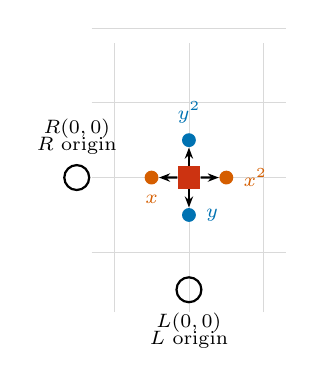
\begin{tikzpicture}[scale=0.95]
  \latwin{-1}{1}{0}{3}
  \node[Xck, minimum size=8pt] (c) at \Xpos{0}{0} {};
  \node[origin, label={[font=\scriptsize, align=center]below:$L(0,0)$\\[-2pt]$L$ origin}] at \Lpos{0}{0} {};
  \node[origin, label={[font=\scriptsize, align=center]above:$R(0,0)$\\[-2pt]$R$ origin}] at \Rpos{0}{0} {};
  \node[Lq, label={[font=\scriptsize, Lc]right:$y$}] (l1) at \Lpos{0}{1} {};
  \node[Lq, label={[font=\scriptsize, Lc]above:$y^2$}] (l2) at \Lpos{0}{2} {};
  \node[Rq, label={[font=\scriptsize, Rc]below:$x$}] (r2) at \Rpos{1}{0} {};
  \node[Rq, label={[font=\scriptsize, Rc]right:$x^2$}] (r3) at \Rpos{2}{0} {};
  \foreach \q in {l1,l2,r2,r3} \draw[link] (c) -- (\q);
\end{tikzpicture}
\caption{Toric X check: $A = y+y^2$, $B = x+x^2$.}
\end{subfigure}\hfill
\begin{subfigure}{0.37\textwidth}\centering
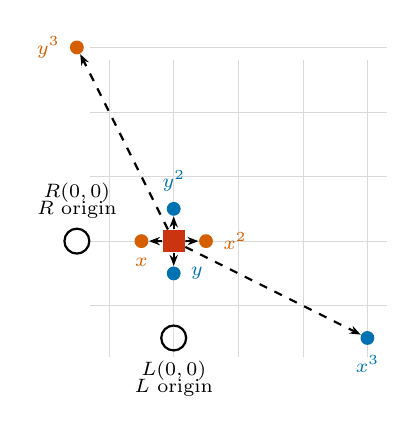
\begin{tikzpicture}[scale=0.82]
  \latwin{-1}{3}{0}{4}
  \node[Xck, minimum size=8pt] (c) at \Xpos{0}{0} {};
  \node[origin, label={[font=\scriptsize, align=center]below:$L(0,0)$\\[-2pt]$L$ origin}] at \Lpos{0}{0} {};
  \node[origin, label={[font=\scriptsize, align=center]above:$R(0,0)$\\[-2pt]$R$ origin}] at \Rpos{0}{0} {};
  \node[Lq, label={[font=\scriptsize, Lc]right:$y$}] (l1) at \Lpos{0}{1} {};
  \node[Lq, label={[font=\scriptsize, Lc]above:$y^2$}] (l2) at \Lpos{0}{2} {};
  \node[Rq, label={[font=\scriptsize, Rc]below:$x$}] (r2) at \Rpos{1}{0} {};
  \node[Rq, label={[font=\scriptsize, Rc]right:$x^2$}] (r3) at \Rpos{2}{0} {};
  \node[Lq, label={[font=\scriptsize, Lc]below:$x^3$}] (l3) at \Lpos{3}{0} {};
  \node[Rq, label={[font=\scriptsize, Rc]left:$y^3$}] (r1) at \Rpos{0}{3} {};
  \foreach \q in {l1,l2,r2,r3} \draw[link] (c) -- (\q);
  \draw[link, dashed] (c) -- (l3);
  \draw[link, dashed] (c) -- (r1);
\end{tikzpicture}
\caption{Gross X check: $A = (y+y^2)+x^3$, $B = (x+x^2)+y^3$.}
\end{subfigure}\hfill
\begin{subfigure}{0.37\textwidth}\centering
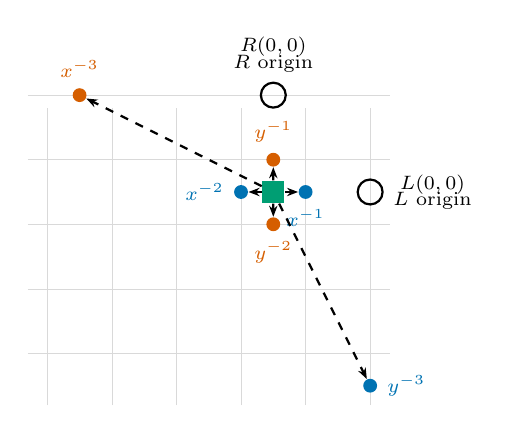
\begin{tikzpicture}[scale=0.82]
  \latwin{-5}{0}{-3}{1}
  \node[Zck, minimum size=8pt] (c) at \Zpos{0}{0} {};
  \node[origin, label={[font=\scriptsize, align=center]right:$L(0,0)$\\[-2pt]$L$ origin}] at \Lpos{0}{0} {};
  \node[origin, label={[font=\scriptsize, align=center]above:$R(0,0)$\\[-2pt]$R$ origin}] at \Rpos{0}{0} {};
  \node[Lq, label={[font=\scriptsize, Lc]below:$x^{-1}$}] (l1) at \Lpos{-1}{0} {};
  \node[Lq, label={[font=\scriptsize, Lc]left:$x^{-2}$}] (l2) at \Lpos{-2}{0} {};
  \node[Rq, label={[font=\scriptsize, Rc]above:$y^{-1}$}] (r1) at \Rpos{0}{-1} {};
  \node[Rq, label={[font=\scriptsize, Rc]below:$y^{-2}$}] (r2) at \Rpos{0}{-2} {};
  \node[Lq, label={[font=\scriptsize, Lc]right:$y^{-3}$}] (l3) at \Lpos{0}{-3} {};
  \node[Rq, label={[font=\scriptsize, Rc]above:$x^{-3}$}] (r3) at \Rpos{-3}{0} {};
  \foreach \q in {l1,l2,r1,r2} \draw[link] (c) -- (\q);
  \draw[link, dashed] (c) -- (l3);
  \draw[link, dashed] (c) -- (r3);
\end{tikzpicture}
\caption{Gross Z check: $B^{-1}$ on $L$, $A^{-1}$ on $R$ (reversed moves).}
\end{subfigure}
\caption{The checks of site $(0,0)$ as stencils (X check: red square on a vertex; Z check: green
square on a face). Black rings: the origins $L(0,0)$ and $R(0,0)$, i.e.\ the monomial $1$; every
arrow is a move \emph{from the ring of its own colour block}: blue $L$ qubits are reached from
$L(0,0)$, orange $R$ qubits from $R(0,0)$. E.g.\ in (b) $x^3$ is the $L$ qubit three steps right of
$L(0,0)$, $y^3$ the $R$ qubit three steps up from $R(0,0)$; in (c) $y^{-3}$ is the $L$ qubit three
steps down from $L(0,0)$. The origins sit 1.5 steps from their check: below and left of an X
check, right of and above a Z check (table in the text).}
\label{fig:stencil}
\end{figure}

\begin{figure}[h]
\centering
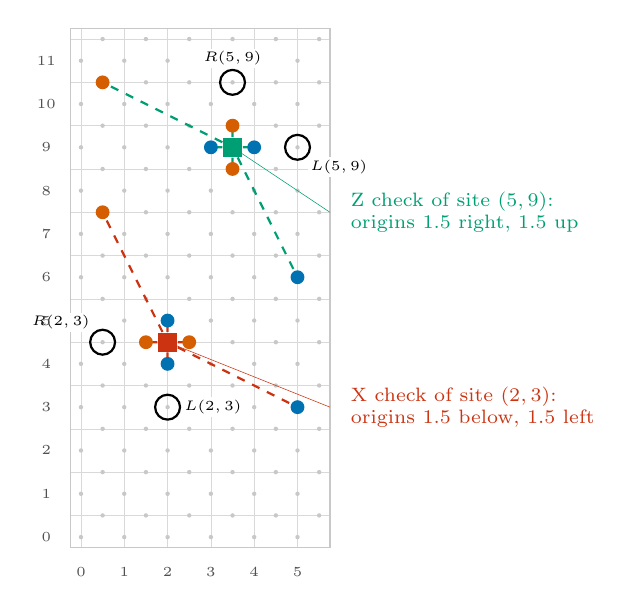
\begin{tikzpicture}[scale=0.55]
  \torus
  % X check at (2,3): local L (2,4),(2,5), R (3,3),(4,3); long L (5,3), R (2,6)
  \node[origin, label={[font=\tiny, fill=white, inner sep=1pt]right:$L(2,3)$}] at \Lpos{2}{3} {};
  \node[origin, label={[font=\tiny, fill=white, inner sep=1pt]above left:$R(2,3)$}] at \Rpos{2}{3} {};
  \node[Xck, minimum size=7pt] (x) at \Xpos{2}{3} {};
  \foreach \a/\b in {2/4,2/5}{\draw[Xc, thick] (x) -- \Lpos{\a}{\b}; \node[Lq] at \Lpos{\a}{\b} {};}
  \foreach \a/\b in {3/3,4/3}{\draw[Xc, thick] (x) -- \Rpos{\a}{\b}; \node[Rq] at \Rpos{\a}{\b} {};}
  \draw[Xc, thick, dashed] (x) -- \Lpos{5}{3}; \node[Lq] at \Lpos{5}{3} {};
  \draw[Xc, thick, dashed] (x) -- \Rpos{2}{6}; \node[Rq] at \Rpos{2}{6} {};
  % Z check at (5,9): local L (4,9),(3,9), R (5,8),(5,7); long L (5,6), R (2,9)
  \node[origin, label={[font=\tiny, fill=white, inner sep=1pt]below right:$L(5,9)$}] at \Lpos{5}{9} {};
  \node[origin, label={[font=\tiny, fill=white, inner sep=1pt]above:$R(5,9)$}] at \Rpos{5}{9} {};
  \node[Zck, minimum size=7pt] (z) at \Zpos{5}{9} {};
  \foreach \a/\b in {4/9,3/9}{\draw[Zc, thick] (z) -- \Lpos{\a}{\b}; \node[Lq] at \Lpos{\a}{\b} {};}
  \foreach \a/\b in {5/8,5/7}{\draw[Zc, thick] (z) -- \Rpos{\a}{\b}; \node[Rq] at \Rpos{\a}{\b} {};}
  \draw[Zc, thick, dashed] (z) -- \Lpos{5}{6}; \node[Lq] at \Lpos{5}{6} {};
  \draw[Zc, thick, dashed] (z) -- \Rpos{2}{9}; \node[Rq] at \Rpos{2}{9} {};
  \node[right=4pt, font=\scriptsize, Xc, align=left] at (5.75,3.0) {X check of site $(2,3)$:\\ origins 1.5 below, 1.5 left};
  \node[right=4pt, font=\scriptsize, Zc, align=left] at (5.75,7.5) {Z check of site $(5,9)$:\\ origins 1.5 right, 1.5 up};
  \draw[Xc, very thin] (5.75,3.0) -- \Xpos{2}{3};
  \draw[Zc, very thin] (5.75,7.5) -- \Zpos{5}{9};
  \foreach \a in {0,...,5} \node[font=\tiny, faint!40!black] at (\a,-0.8) {\a};
  \foreach \b in {0,...,11} \node[font=\tiny, faint!40!black] at (-0.8,\b) {\b};
\end{tikzpicture}
\caption{The whole gross code ($x$ right, $y$ up; tick labels are $a$ and $b$) with two checks
drawn. Each touches the four edges around it (solid) and two distant qubits (dashed); black
rings mark the origins of its site, labelled $L(a,b)$ and $R(a,b)$: the X check of site $(2,3)$
moves from $L(2,3)$ and $R(2,3)$, the Z check of site $(5,9)$ from $L(5,9)$ and $R(5,9)$. The X check uses $A$ from the $L$ origin and $B$
from the $R$ origin; the Z check uses the reversed moves, $B^{-1}$ on $L$ and $A^{-1}$ on $R$.
Checks near the border have legs that wrap around the torus.}
\label{fig:full}
\end{figure}

\paragraph{Gross = toric + two long legs.} Drop $x^3$ and $y^3$ and you are left with
$A = y(1+y)$, $B = x(1+x)$. Up to a relabelling of qubits (the monomial factors $y$, $x$ are just
shifts), this is the toric code $A=1+y$, $B=1+x$, whose checks are the four nearest edges
(\cref{fig:stencil}a). The gross code keeps the same idea, ``one stencil copied
everywhere'', and adds one long leg on each block. The long legs $x^3$ and $y^3$ are what makes the code
non-local on a 2D chip, and also what buys $k=12$ logical qubits and distance $12$ from only
144 qubits (the toric code needs 288 qubits for $k=2$, $d=12$).

\subsection{Why X and Z checks commute}
A Z check and an X check must overlap on an even number of qubits. In matrix form,
$H_X H_Z^{\mathsf T} = AB + BA = 2AB = 0$, because shifts commute ($AB=BA$). The picture
behind this (\cref{fig:commute}): the X check at $\alpha$ reaches $L$ qubit $\alpha+u$ for
$u\in A$, and the Z check at $\beta$ reaches $L$ qubit $\beta-v$ for $v\in B$. They meet on
$L$ when $\beta-\alpha = u+v$. On $R$ the X check moves by $v\in B$ and the Z check back by
$u\in A$, so they meet when $\beta-\alpha = v+u$, the same condition. Every shared $L$ qubit
comes with a shared $R$ qubit: ``first $u$ then $v$'' versus ``first $v$ then $u$''.

\begin{figure}[h]
\centering
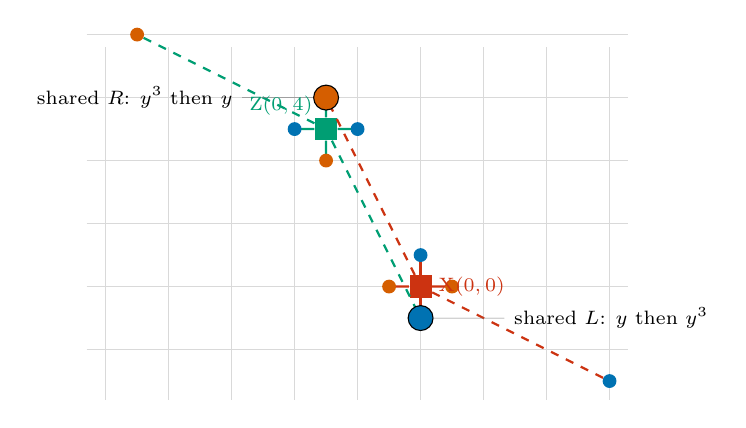
\begin{tikzpicture}[scale=0.8]
  \latwin{-5}{3}{0}{5}
  % X check at (0,0): local L (0,1),(0,2), R (1,0),(2,0); long L (3,0), R (0,3)
  \node[Xck, minimum size=8pt] (x) at \Xpos{0}{0} {};
  \draw[Xc, thick] (x) -- \Lpos{0}{2}; \node[Lq] at \Lpos{0}{2} {};
  \foreach \a/\b in {1/0, 2/0} {\draw[Xc, thick] (x) -- \Rpos{\a}{\b}; \node[Rq] at \Rpos{\a}{\b} {};}
  \draw[Xc, thick, dashed] (x) -- \Lpos{3}{0}; \node[Lq] at \Lpos{3}{0} {};
  % Z check at (0,4): local L (-1,4),(-2,4), R (0,3),(0,2); long L (0,1), R (-3,4)
  \node[Zck, minimum size=8pt] (z) at \Zpos{0}{4} {};
  \foreach \a/\b in {-1/4, -2/4} {\draw[Zc, thick] (z) -- \Lpos{\a}{\b}; \node[Lq] at \Lpos{\a}{\b} {};}
  \draw[Zc, thick] (z) -- \Rpos{0}{2}; \node[Rq] at \Rpos{0}{2} {};
  \draw[Zc, thick, dashed] (z) -- \Rpos{-3}{4}; \node[Rq] at \Rpos{-3}{4} {};
  % shared: L (0,1) = X local + Z long;  R (0,3) = X long + Z local
  \draw[Xc, thick] (x) -- \Lpos{0}{1};  \draw[Zc, thick, dashed] (z) -- \Lpos{0}{1};
  \draw[Xc, thick, dashed] (x) -- \Rpos{0}{3}; \draw[Zc, thick] (z) -- \Rpos{0}{3};
  \node[Lq, minimum size=9pt, draw=black, pin={[font=\scriptsize, pin distance=9mm]right:shared $L$: $y$ then $y^3$}] at \Lpos{0}{1} {};
  \node[Rq, minimum size=9pt, draw=black, pin={[font=\scriptsize, pin distance=9mm]left:shared $R$: $y^3$ then $y$}] at \Rpos{0}{3} {};
  \node[right=3pt, font=\scriptsize, Xc] at \Xpos{0}{0} {X$(0,0)$};
  \node[above left=2pt, font=\scriptsize, Zc] at \Zpos{0}{4} {Z$(0,4)$};
\end{tikzpicture}
\caption{The X check at $(0,0)$ and the Z check at $(0,4)$ share exactly two qubits, one $L$
and one $R$. Their offset $y^4 = y\cdot y^3$ can be split as ``$y\in A$ then $y^3\in B$'' (meeting
on $L$: a local leg of X, a long leg of Z) or ``$y^3\in B$ then $y\in A$'' (meeting on $R$: a long
leg of X, a local leg of Z).}
\label{fig:commute}
\end{figure}

%======================================================================
\section{Checking an error: three questions}

Let $e\in\F^{144}$ be an X error, $e_q = 1$ if qubit $q$ is flipped. In a decoder
evaluation, $e$ is the \emph{residual}: true error plus the decoder's correction.

\begin{figure}[h]
\centering
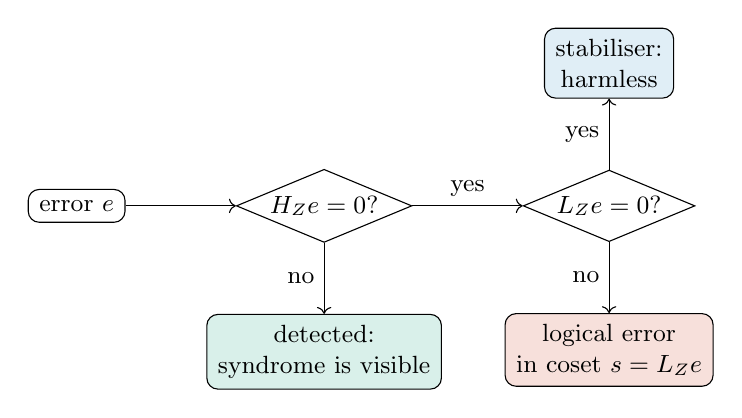
\begin{tikzpicture}[node distance=0.9cm and 1.4cm, font=\small,
    box/.style={draw, rounded corners, align=center, inner sep=4pt},
    q/.style={draw, diamond, aspect=2.4, align=center, inner sep=1pt}]
  \node[box] (e) {error $e$};
  \node[q, right=of e] (q1) {$H_Z e = 0$?};
  \node[q, right=of q1] (q2) {$L_Z e = 0$?};
  \node[box, below=of q1, fill=Zc!15] (det) {detected:\\ syndrome is visible};
  \node[box, above=of q2, fill=Lc!12] (stab) {stabiliser:\\ harmless};
  \node[box, below=of q2, fill=Xc!15] (log) {logical error\\ in coset $s = L_Z e$};
  \draw[->] (e) -- (q1);
  \draw[->] (q1) -- node[above] {yes} (q2);
  \draw[->] (q1) -- node[left] {no} (det);
  \draw[->] (q2) -- node[left] {yes} (stab);
  \draw[->] (q2) -- node[left] {no} (log);
\end{tikzpicture}
\caption{Classifying an X error. Both tests are one matrix--vector product mod 2.}
\label{fig:flow}
\end{figure}

\begin{enumerate}
\item \textbf{Is it detected?} The syndrome is $\sigma = H_Z e$: Z check $j$ fires iff it
      overlaps $e$ on an odd number of qubits. If $\sigma\neq 0$ the decoder sees the
      error.
\item \textbf{Is it harmless?} If $\sigma = 0$, the error is invisible. Invisible errors are
      either products of X checks (stabilisers, they do nothing to the encoded state) or
      logical operators (they do). Example: the stencil of one X check, used as an error, is
      invisible \emph{and} harmless; it has weight 6.
\item \textbf{Which logical error?} Take $L_Z$, $12$ Z-type logical operators
      (a basis of $\ker H_X$ modulo $\rowsp H_Z$). Each one is a ``probe'' that commutes
      with all checks; it anticommutes with $e$ iff $e$ flips that logical qubit. The
      \emph{coset} of $e$ is
      \[ s = L_Z\, e \in \F^{12}. \]
      $s=0$ means stabiliser; $s\neq 0$ is a logical error, and bit $i$ of $s$ says whether
      logical qubit $i$ was flipped. We store $s$ as the integer $c=\sum_i s_i 2^i$, the
      \emph{coset id}.
\end{enumerate}

Two invisible errors with the same $s$ differ by a stabiliser, so they are the same error as
far as the encoded information is concerned: a coset is a whole family of equivalent
patterns. There are $2^{12}-1 = 4095$ non-trivial X cosets. (The count of logical qubits:
$k = n - \rk H_X - \rk H_Z = 144-66-66 = 12$.)

%======================================================================
\section{An example: a weight-12 logical}

The distance is $12$: no invisible, non-trivial error is lighter. \Cref{fig:logical} shows
one that reaches this bound. It flips only $L$ qubits, at
\[
  f(x,y) = (1+y^6)\,\bigl(1 + x^2 + y^3(x+x^2+x^3+x^4)\bigr),
\]
i.e.\ each monomial $x^ay^b$ of $f$ is a flipped qubit at $(a,b)$.

\begin{figure}[h]
\centering
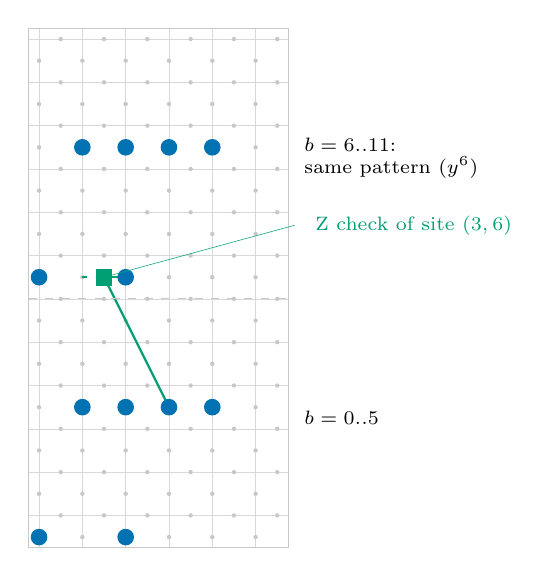
\begin{tikzpicture}[scale=0.55]
  \torus
  % Z check (3,6): L legs (B^T) at (2,6), (1,6) [local], (3,3) [long]
  \draw[Zc, thick] \Zpos{3}{6} -- \Lpos{2}{6};
  \draw[Zc, thick, dashed] \Zpos{3}{6} -- \Lpos{1}{6};
  \draw[Zc, thick] \Zpos{3}{6} -- \Lpos{3}{3};
  \foreach \a/\b in {0/0,0/6,1/3,1/9,2/0,2/3,2/6,2/9,3/3,3/9,4/3,4/9}
    \node[Lq, minimum size=6pt] at \LposT{\a}{\b} {};
  \node[Zck, minimum size=6pt] at \Zpos{3}{6} {};
  \draw[faint, dashed] (-0.25,5.5) -- (5.75,5.5);
  \node[right, font=\scriptsize] at (5.9,2.75) {$b=0..5$};
  \node[right, font=\scriptsize, align=left] at (5.9,8.75) {$b=6..11$:\\ same pattern ($y^6$)};
  \node[right=4pt, font=\scriptsize, Zc] at (5.9,7.2) {Z check of site $(3,6)$};
  \draw[Zc, very thin] (5.9,7.2) -- \Zpos{3}{6};
\end{tikzpicture}
\caption{A weight-12 logical X error (coset id 128). Blue: flipped $L$ qubits. Green: the three $L$
legs of the Z check of site $(3,6)$ (moves $x^{-1}, x^{-2}$ to the edges left and right of it,
$y^{-3}$ far down; the dashed leg ends on an unflipped qubit).
It overlaps the error on two qubits, so it does not fire. All 18 Z checks that touch the
pattern overlap it on exactly two qubits, so the syndrome is zero.}
\label{fig:logical}
\end{figure}

\paragraph{Polynomial view.} For an error $f$ on $L$ only, the Z checks see it through
$B^{\mathsf T}$, which in polynomial language is multiplication by $B$. So
\[
  \text{$f$ on $L$ is invisible} \iff B(x,y)\, f(x,y) = 0 \quad\text{in } \F[x,y]/(x^6-1,\,y^{12}-1).
\]
This is a ``null space'' condition on a much smaller space (only 72 unknowns), and the
null space has dimension 12: one can list \emph{all} $2^{12}=4096$ $L$-only invisible errors
in a tenth of a second. Of these, 36 have weight 12, and they are exactly the 36 shifts of
\cref{fig:logical} (see next section).

%======================================================================
\section{Orbits: the same pattern, shifted}

Shifting every qubit by the same move $x^iy^j$ maps checks to checks (every check is the
same stencil). So a shifted logical is still invisible and has the same weight and shape,
but it is in general a \emph{different coset}: it flips a different combination of the 12
logical qubits (\cref{fig:orbit}). All cosets obtained from one by shifting form an
\emph{orbit}.

\newcommand{\minilogical}[3]{% #1 = da, #2 = db, #3 = caption
\begin{tikzpicture}[scale=0.24]
  \torus
  \foreach \a/\b in {0/0,0/6,1/3,1/9,2/0,2/3,2/6,2/9,3/3,3/9,4/3,4/9}{
    \pgfmathtruncatemacro{\aa}{mod(\a+#1,6)}\pgfmathtruncatemacro{\bb}{mod(\b+#2,12)}
    \node[Lq, minimum size=3.4pt] at \LposT{\aa}{\bb} {};}
  \node[font=\scriptsize] at (2.75,-1.3) {#3};
\end{tikzpicture}}
\begin{figure}[h]
\centering
\minilogical{0}{0}{$f$: coset 128}\hfill
\minilogical{0}{1}{$y f$: coset 3008}\hfill
\minilogical{1}{0}{$x f$: coset 2048}\hfill
\minilogical{0}{6}{$y^6 f$: coset 128}
\caption{One orbit. Shifting the logical of \cref{fig:logical} by $y$ or by $x$ gives
other cosets; shifting by $y^6$ gives the \emph{same} pattern back, because
$f = (1+y^6)(\dots)$. Of the $72$ shifts, pairs give the same coset, so this orbit has
$72/2 = 36$ cosets.}
\label{fig:orbit}
\end{figure}

In general the orbit size is $72/|\mathrm{Stab}|$, with $|\mathrm{Stab}|$ the number of shifts
that leave the coset unchanged. For the gross code the 4095 cosets fall into \textbf{155
orbits} of sizes 3, 9, 12 and 36. One representative per orbit is enough to see every
distinct shape. Computing the orbits needs no optimisation: take \emph{any} representative
of a coset (from a basis of X logicals), shift it 72 times, read off $L_Z$ of each copy.

%======================================================================
\section{Finding the lightest representative of each orbit}

Finding \emph{some} invisible non-trivial error is a null-space computation. Finding the
\emph{lightest} one in a given coset is hard:
\[
  \min |e| \quad\text{s.t.}\quad H_Z e = 0,\ L_Z e = s .
\]
The full null space $\ker H_Z$ has dimension $144-66 = 78$, i.e.\ $2^{78}\approx
3\cdot 10^{23}$ vectors, far too many to list, and the minimum-weight problem for linear codes
is NP-hard in general. Three practical routes:

\paragraph{1. Single-block null spaces (instant, exact, partial).}
As in the previous section: errors on $L$ only need $Bf=0$, errors on $R$ only need $Ag=0$.
Each null space has dimension 12 and is listed completely:

\begin{center}
\begin{tabular}{lccc}
\toprule
block & null space dim & weight-12 logicals & weight-16 logicals \\
\midrule
$L$ only & 12 & 36 words $\to$ 36 cosets (one orbit) & 9 words $\to$ 3 cosets \\
$R$ only & 12 & 36 words $\to$ 36 cosets (same orbit) & 9 words $\to$ 3 cosets \\
\bottomrule
\end{tabular}
\end{center}
Patterns that use both blocks are not covered.

\paragraph{2. Information-set sampling (fast, no proof).}
Let $G$ ($78\times 144$) be a basis of $\ker H_Z$. A trial: shuffle the 144 columns, row-reduce
$G$. Each row now has a single 1 on 78 ``pivot'' columns and is free elsewhere. Every row, and
every sum of two rows, is an invisible error with at most two 1s on the pivots; keep the light
ones with $L_Z e\ne 0$. A fixed pattern of weight $w$ is caught in one trial with probability
\[
  P_w = \sum_{j=0}^{2}\binom{78}{j}\binom{66}{w-j}\Big/\binom{144}{w},
  \qquad P_{12}\approx 7.0\cdot 10^{-3},\quad P_{14}\approx 1.7\cdot 10^{-3},
\]
i.e.\ about 140 (resp.\ 600) trials per pattern, at a few milliseconds per trial. This gives
many orbits quickly. It only gives upper bounds: not finding an orbit proves nothing.

\paragraph{3. Exact integer program (slow, certified).}
Write each mod-2 equation as an integer one with a slack, $r\cdot e - 2t = \text{rhs}$, and
minimise $\sum_q e_q$ (HiGHS, zero optimality gap). Closing the gap is a proof of minimality.
Easy orbits (weight 12) take about a minute; proving that a coset has \emph{no}
representative of weight $\le 14$ often takes more than 10 minutes. Use it to certify a
few orbits, not to scan all 155.

%======================================================================
\section{What the lowest-weight logicals look like}

A run of information-set sampling (20\,000 trials, 2 workers, 4 minutes; weights up to 16)
found representatives for 95 of the 155 orbits:

\begin{center}
\begin{tabular}{rrrl}
\toprule
weight & orbits & cosets covered & status \\
\midrule
12 & 9  & 246  & minimal (distance bound) \\
14 & 26 & 888  & upper bound \\
16 & 60 & 1701 & upper bound \\
$>16$? & 60 & 1260 & not seen \\
\bottomrule
\end{tabular}
\end{center}
No new orbit appeared after the first $\sim$1000 trials, while each weight-12 pattern is
expected about every 140 trials; the 60 orbits never seen are very likely heavier than 16, but
this is not a proof. \Cref{fig:found} draws one representative per orbit: all nine of weight 12
and nine of the 26 of weight 14, each shifted to a compact position.

\begin{figure}[h]
\centering
% generated from results/cosets/144_12_12_ldpc/enum_catalogue.csv
\par\medskip\noindent
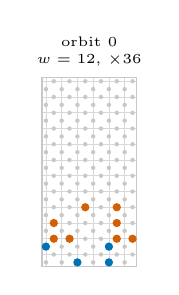
\begin{tikzpicture}[scale=0.2]
  \torus
  \node[Lq, minimum size=3pt] at \LposT{0}{1} {};
  \node[Lq, minimum size=3pt] at \LposT{2}{0} {};
  \node[Lq, minimum size=3pt] at \LposT{4}{0} {};
  \node[Lq, minimum size=3pt] at \LposT{4}{1} {};
  \node[Rq, minimum size=3pt] at \RposT{0}{0} {};
  \node[Rq, minimum size=3pt] at \RposT{0}{1} {};
  \node[Rq, minimum size=3pt] at \RposT{0}{2} {};
  \node[Rq, minimum size=3pt] at \RposT{1}{0} {};
  \node[Rq, minimum size=3pt] at \RposT{2}{0} {};
  \node[Rq, minimum size=3pt] at \RposT{2}{1} {};
  \node[Rq, minimum size=3pt] at \RposT{3}{0} {};
  \node[Rq, minimum size=3pt] at \RposT{4}{2} {};
  \node[font=\tiny, align=center] at (2.75,13.4) {orbit 0\\ $w=12$, $\times36$};
\end{tikzpicture}\hfill
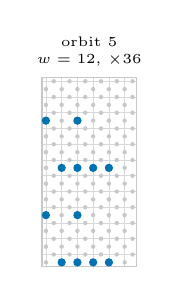
\begin{tikzpicture}[scale=0.2]
  \torus
  \node[Lq, minimum size=3pt] at \LposT{0}{3} {};
  \node[Lq, minimum size=3pt] at \LposT{0}{9} {};
  \node[Lq, minimum size=3pt] at \LposT{1}{0} {};
  \node[Lq, minimum size=3pt] at \LposT{1}{6} {};
  \node[Lq, minimum size=3pt] at \LposT{2}{0} {};
  \node[Lq, minimum size=3pt] at \LposT{2}{3} {};
  \node[Lq, minimum size=3pt] at \LposT{2}{6} {};
  \node[Lq, minimum size=3pt] at \LposT{2}{9} {};
  \node[Lq, minimum size=3pt] at \LposT{3}{0} {};
  \node[Lq, minimum size=3pt] at \LposT{3}{6} {};
  \node[Lq, minimum size=3pt] at \LposT{4}{0} {};
  \node[Lq, minimum size=3pt] at \LposT{4}{6} {};
  \node[font=\tiny, align=center] at (2.75,13.4) {orbit 5\\ $w=12$, $\times36$};
\end{tikzpicture}\hfill
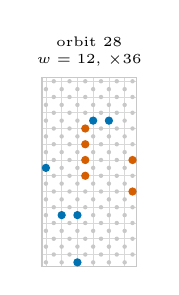
\begin{tikzpicture}[scale=0.2]
  \torus
  \node[Lq, minimum size=3pt] at \LposT{0}{6} {};
  \node[Lq, minimum size=3pt] at \LposT{1}{3} {};
  \node[Lq, minimum size=3pt] at \LposT{2}{0} {};
  \node[Lq, minimum size=3pt] at \LposT{2}{3} {};
  \node[Lq, minimum size=3pt] at \LposT{3}{9} {};
  \node[Lq, minimum size=3pt] at \LposT{4}{9} {};
  \node[Rq, minimum size=3pt] at \RposT{1}{3} {};
  \node[Rq, minimum size=3pt] at \RposT{1}{5} {};
  \node[Rq, minimum size=3pt] at \RposT{4}{4} {};
  \node[Rq, minimum size=3pt] at \RposT{4}{5} {};
  \node[Rq, minimum size=3pt] at \RposT{4}{6} {};
  \node[Rq, minimum size=3pt] at \RposT{4}{7} {};
  \node[font=\tiny, align=center] at (2.75,13.4) {orbit 28\\ $w=12$, $\times36$};
\end{tikzpicture}\hfill
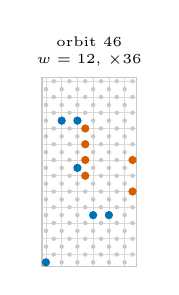
\begin{tikzpicture}[scale=0.2]
  \torus
  \node[Lq, minimum size=3pt] at \LposT{0}{0} {};
  \node[Lq, minimum size=3pt] at \LposT{1}{9} {};
  \node[Lq, minimum size=3pt] at \LposT{2}{6} {};
  \node[Lq, minimum size=3pt] at \LposT{2}{9} {};
  \node[Lq, minimum size=3pt] at \LposT{3}{3} {};
  \node[Lq, minimum size=3pt] at \LposT{4}{3} {};
  \node[Rq, minimum size=3pt] at \RposT{1}{3} {};
  \node[Rq, minimum size=3pt] at \RposT{1}{5} {};
  \node[Rq, minimum size=3pt] at \RposT{4}{4} {};
  \node[Rq, minimum size=3pt] at \RposT{4}{5} {};
  \node[Rq, minimum size=3pt] at \RposT{4}{6} {};
  \node[Rq, minimum size=3pt] at \RposT{4}{7} {};
  \node[font=\tiny, align=center] at (2.75,13.4) {orbit 46\\ $w=12$, $\times36$};
\end{tikzpicture}\hfill
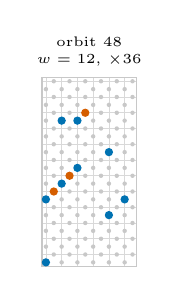
\begin{tikzpicture}[scale=0.2]
  \torus
  \node[Lq, minimum size=3pt] at \LposT{0}{0} {};
  \node[Lq, minimum size=3pt] at \LposT{0}{4} {};
  \node[Lq, minimum size=3pt] at \LposT{1}{5} {};
  \node[Lq, minimum size=3pt] at \LposT{1}{9} {};
  \node[Lq, minimum size=3pt] at \LposT{2}{6} {};
  \node[Lq, minimum size=3pt] at \LposT{2}{9} {};
  \node[Lq, minimum size=3pt] at \LposT{4}{3} {};
  \node[Lq, minimum size=3pt] at \LposT{4}{7} {};
  \node[Lq, minimum size=3pt] at \LposT{5}{4} {};
  \node[Rq, minimum size=3pt] at \RposT{2}{3} {};
  \node[Rq, minimum size=3pt] at \RposT{3}{4} {};
  \node[Rq, minimum size=3pt] at \RposT{4}{8} {};
  \node[font=\tiny, align=center] at (2.75,13.4) {orbit 48\\ $w=12$, $\times36$};
\end{tikzpicture}\hfill
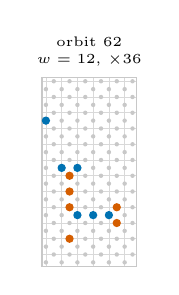
\begin{tikzpicture}[scale=0.2]
  \torus
  \node[Lq, minimum size=3pt] at \LposT{0}{9} {};
  \node[Lq, minimum size=3pt] at \LposT{1}{6} {};
  \node[Lq, minimum size=3pt] at \LposT{2}{3} {};
  \node[Lq, minimum size=3pt] at \LposT{2}{6} {};
  \node[Lq, minimum size=3pt] at \LposT{3}{3} {};
  \node[Lq, minimum size=3pt] at \LposT{4}{3} {};
  \node[Rq, minimum size=3pt] at \RposT{0}{1} {};
  \node[Rq, minimum size=3pt] at \RposT{0}{2} {};
  \node[Rq, minimum size=3pt] at \RposT{3}{0} {};
  \node[Rq, minimum size=3pt] at \RposT{3}{2} {};
  \node[Rq, minimum size=3pt] at \RposT{3}{3} {};
  \node[Rq, minimum size=3pt] at \RposT{3}{4} {};
  \node[font=\tiny, align=center] at (2.75,13.4) {orbit 62\\ $w=12$, $\times36$};
\end{tikzpicture}\hfill
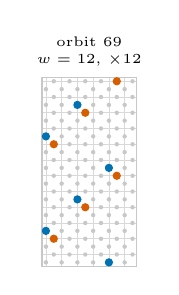
\begin{tikzpicture}[scale=0.2]
  \torus
  \node[Lq, minimum size=3pt] at \LposT{0}{2} {};
  \node[Lq, minimum size=3pt] at \LposT{0}{8} {};
  \node[Lq, minimum size=3pt] at \LposT{2}{4} {};
  \node[Lq, minimum size=3pt] at \LposT{2}{10} {};
  \node[Lq, minimum size=3pt] at \LposT{4}{0} {};
  \node[Lq, minimum size=3pt] at \LposT{4}{6} {};
  \node[Rq, minimum size=3pt] at \RposT{0}{4} {};
  \node[Rq, minimum size=3pt] at \RposT{0}{10} {};
  \node[Rq, minimum size=3pt] at \RposT{2}{0} {};
  \node[Rq, minimum size=3pt] at \RposT{2}{6} {};
  \node[Rq, minimum size=3pt] at \RposT{4}{2} {};
  \node[Rq, minimum size=3pt] at \RposT{4}{8} {};
  \node[font=\tiny, align=center] at (2.75,13.4) {orbit 69\\ $w=12$, $\times12$};
\end{tikzpicture}\hfill
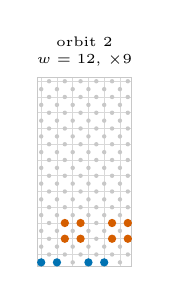
\begin{tikzpicture}[scale=0.2]
  \torus
  \node[Lq, minimum size=3pt] at \LposT{0}{0} {};
  \node[Lq, minimum size=3pt] at \LposT{1}{0} {};
  \node[Lq, minimum size=3pt] at \LposT{3}{0} {};
  \node[Lq, minimum size=3pt] at \LposT{4}{0} {};
  \node[Rq, minimum size=3pt] at \RposT{0}{0} {};
  \node[Rq, minimum size=3pt] at \RposT{0}{1} {};
  \node[Rq, minimum size=3pt] at \RposT{1}{0} {};
  \node[Rq, minimum size=3pt] at \RposT{1}{1} {};
  \node[Rq, minimum size=3pt] at \RposT{3}{0} {};
  \node[Rq, minimum size=3pt] at \RposT{3}{1} {};
  \node[Rq, minimum size=3pt] at \RposT{4}{0} {};
  \node[Rq, minimum size=3pt] at \RposT{4}{1} {};
  \node[font=\tiny, align=center] at (2.75,13.4) {orbit 2\\ $w=12$, $\times9$};
\end{tikzpicture}\hfill
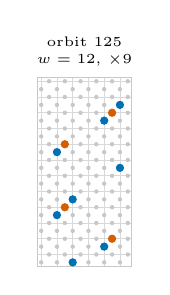
\begin{tikzpicture}[scale=0.2]
  \torus
  \node[Lq, minimum size=3pt] at \LposT{1}{3} {};
  \node[Lq, minimum size=3pt] at \LposT{1}{7} {};
  \node[Lq, minimum size=3pt] at \LposT{2}{0} {};
  \node[Lq, minimum size=3pt] at \LposT{2}{4} {};
  \node[Lq, minimum size=3pt] at \LposT{4}{1} {};
  \node[Lq, minimum size=3pt] at \LposT{4}{9} {};
  \node[Lq, minimum size=3pt] at \LposT{5}{6} {};
  \node[Lq, minimum size=3pt] at \LposT{5}{10} {};
  \node[Rq, minimum size=3pt] at \RposT{0}{0} {};
  \node[Rq, minimum size=3pt] at \RposT{0}{8} {};
  \node[Rq, minimum size=3pt] at \RposT{3}{2} {};
  \node[Rq, minimum size=3pt] at \RposT{3}{6} {};
  \node[font=\tiny, align=center] at (2.75,13.4) {orbit 125\\ $w=12$, $\times9$};
\end{tikzpicture}
\par\medskip\noindent
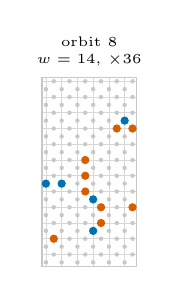
\begin{tikzpicture}[scale=0.2]
  \torus
  \node[Lq, minimum size=3pt] at \LposT{0}{5} {};
  \node[Lq, minimum size=3pt] at \LposT{1}{5} {};
  \node[Lq, minimum size=3pt] at \LposT{3}{2} {};
  \node[Lq, minimum size=3pt] at \LposT{3}{4} {};
  \node[Lq, minimum size=3pt] at \LposT{5}{9} {};
  \node[Rq, minimum size=3pt] at \RposT{0}{7} {};
  \node[Rq, minimum size=3pt] at \RposT{1}{2} {};
  \node[Rq, minimum size=3pt] at \RposT{1}{7} {};
  \node[Rq, minimum size=3pt] at \RposT{2}{0} {};
  \node[Rq, minimum size=3pt] at \RposT{4}{3} {};
  \node[Rq, minimum size=3pt] at \RposT{4}{4} {};
  \node[Rq, minimum size=3pt] at \RposT{4}{5} {};
  \node[Rq, minimum size=3pt] at \RposT{5}{1} {};
  \node[Rq, minimum size=3pt] at \RposT{5}{2} {};
  \node[font=\tiny, align=center] at (2.75,13.4) {orbit 8\\ $w=14$, $\times36$};
\end{tikzpicture}\hfill
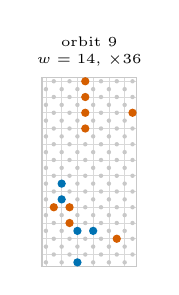
\begin{tikzpicture}[scale=0.2]
  \torus
  \node[Lq, minimum size=3pt] at \LposT{1}{4} {};
  \node[Lq, minimum size=3pt] at \LposT{1}{5} {};
  \node[Lq, minimum size=3pt] at \LposT{2}{0} {};
  \node[Lq, minimum size=3pt] at \LposT{2}{2} {};
  \node[Lq, minimum size=3pt] at \LposT{3}{2} {};
  \node[Rq, minimum size=3pt] at \RposT{0}{0} {};
  \node[Rq, minimum size=3pt] at \RposT{1}{8} {};
  \node[Rq, minimum size=3pt] at \RposT{2}{2} {};
  \node[Rq, minimum size=3pt] at \RposT{3}{1} {};
  \node[Rq, minimum size=3pt] at \RposT{3}{2} {};
  \node[Rq, minimum size=3pt] at \RposT{4}{7} {};
  \node[Rq, minimum size=3pt] at \RposT{4}{8} {};
  \node[Rq, minimum size=3pt] at \RposT{4}{9} {};
  \node[Rq, minimum size=3pt] at \RposT{4}{10} {};
  \node[font=\tiny, align=center] at (2.75,13.4) {orbit 9\\ $w=14$, $\times36$};
\end{tikzpicture}\hfill
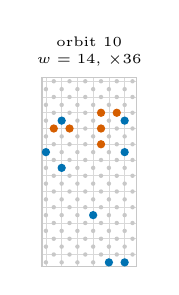
\begin{tikzpicture}[scale=0.2]
  \torus
  \node[Lq, minimum size=3pt] at \LposT{0}{7} {};
  \node[Lq, minimum size=3pt] at \LposT{1}{6} {};
  \node[Lq, minimum size=3pt] at \LposT{1}{9} {};
  \node[Lq, minimum size=3pt] at \LposT{3}{3} {};
  \node[Lq, minimum size=3pt] at \LposT{4}{0} {};
  \node[Lq, minimum size=3pt] at \LposT{5}{0} {};
  \node[Lq, minimum size=3pt] at \LposT{5}{7} {};
  \node[Lq, minimum size=3pt] at \LposT{5}{9} {};
  \node[Rq, minimum size=3pt] at \RposT{0}{8} {};
  \node[Rq, minimum size=3pt] at \RposT{2}{7} {};
  \node[Rq, minimum size=3pt] at \RposT{3}{7} {};
  \node[Rq, minimum size=3pt] at \RposT{5}{6} {};
  \node[Rq, minimum size=3pt] at \RposT{5}{7} {};
  \node[Rq, minimum size=3pt] at \RposT{5}{8} {};
  \node[font=\tiny, align=center] at (2.75,13.4) {orbit 10\\ $w=14$, $\times36$};
\end{tikzpicture}\hfill
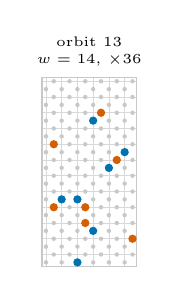
\begin{tikzpicture}[scale=0.2]
  \torus
  \node[Lq, minimum size=3pt] at \LposT{1}{4} {};
  \node[Lq, minimum size=3pt] at \LposT{2}{0} {};
  \node[Lq, minimum size=3pt] at \LposT{2}{4} {};
  \node[Lq, minimum size=3pt] at \LposT{3}{2} {};
  \node[Lq, minimum size=3pt] at \LposT{3}{9} {};
  \node[Lq, minimum size=3pt] at \LposT{4}{6} {};
  \node[Lq, minimum size=3pt] at \LposT{5}{7} {};
  \node[Rq, minimum size=3pt] at \RposT{0}{5} {};
  \node[Rq, minimum size=3pt] at \RposT{1}{0} {};
  \node[Rq, minimum size=3pt] at \RposT{2}{2} {};
  \node[Rq, minimum size=3pt] at \RposT{2}{6} {};
  \node[Rq, minimum size=3pt] at \RposT{4}{1} {};
  \node[Rq, minimum size=3pt] at \RposT{4}{2} {};
  \node[Rq, minimum size=3pt] at \RposT{5}{8} {};
  \node[font=\tiny, align=center] at (2.75,13.4) {orbit 13\\ $w=14$, $\times36$};
\end{tikzpicture}\hfill
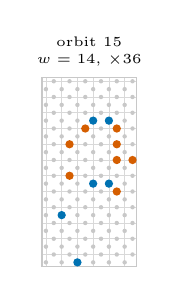
\begin{tikzpicture}[scale=0.2]
  \torus
  \node[Lq, minimum size=3pt] at \LposT{1}{3} {};
  \node[Lq, minimum size=3pt] at \LposT{2}{0} {};
  \node[Lq, minimum size=3pt] at \LposT{3}{5} {};
  \node[Lq, minimum size=3pt] at \LposT{3}{9} {};
  \node[Lq, minimum size=3pt] at \LposT{4}{5} {};
  \node[Lq, minimum size=3pt] at \LposT{4}{9} {};
  \node[Rq, minimum size=3pt] at \RposT{0}{3} {};
  \node[Rq, minimum size=3pt] at \RposT{0}{5} {};
  \node[Rq, minimum size=3pt] at \RposT{0}{6} {};
  \node[Rq, minimum size=3pt] at \RposT{0}{7} {};
  \node[Rq, minimum size=3pt] at \RposT{1}{5} {};
  \node[Rq, minimum size=3pt] at \RposT{3}{4} {};
  \node[Rq, minimum size=3pt] at \RposT{3}{6} {};
  \node[Rq, minimum size=3pt] at \RposT{4}{7} {};
  \node[font=\tiny, align=center] at (2.75,13.4) {orbit 15\\ $w=14$, $\times36$};
\end{tikzpicture}\hfill
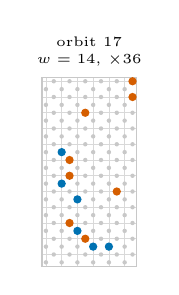
\begin{tikzpicture}[scale=0.2]
  \torus
  \node[Lq, minimum size=3pt] at \LposT{1}{5} {};
  \node[Lq, minimum size=3pt] at \LposT{1}{7} {};
  \node[Lq, minimum size=3pt] at \LposT{2}{2} {};
  \node[Lq, minimum size=3pt] at \LposT{2}{4} {};
  \node[Lq, minimum size=3pt] at \LposT{3}{1} {};
  \node[Lq, minimum size=3pt] at \LposT{4}{1} {};
  \node[Rq, minimum size=3pt] at \RposT{0}{3} {};
  \node[Rq, minimum size=3pt] at \RposT{1}{9} {};
  \node[Rq, minimum size=3pt] at \RposT{1}{10} {};
  \node[Rq, minimum size=3pt] at \RposT{3}{1} {};
  \node[Rq, minimum size=3pt] at \RposT{3}{4} {};
  \node[Rq, minimum size=3pt] at \RposT{3}{5} {};
  \node[Rq, minimum size=3pt] at \RposT{4}{0} {};
  \node[Rq, minimum size=3pt] at \RposT{4}{8} {};
  \node[font=\tiny, align=center] at (2.75,13.4) {orbit 17\\ $w=14$, $\times36$};
\end{tikzpicture}\hfill
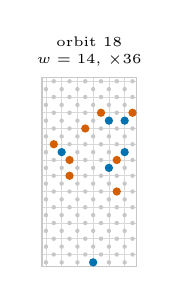
\begin{tikzpicture}[scale=0.2]
  \torus
  \node[Lq, minimum size=3pt] at \LposT{1}{7} {};
  \node[Lq, minimum size=3pt] at \LposT{3}{0} {};
  \node[Lq, minimum size=3pt] at \LposT{4}{6} {};
  \node[Lq, minimum size=3pt] at \LposT{4}{9} {};
  \node[Lq, minimum size=3pt] at \LposT{5}{7} {};
  \node[Lq, minimum size=3pt] at \LposT{5}{9} {};
  \node[Rq, minimum size=3pt] at \RposT{0}{3} {};
  \node[Rq, minimum size=3pt] at \RposT{0}{5} {};
  \node[Rq, minimum size=3pt] at \RposT{1}{8} {};
  \node[Rq, minimum size=3pt] at \RposT{2}{6} {};
  \node[Rq, minimum size=3pt] at \RposT{3}{4} {};
  \node[Rq, minimum size=3pt] at \RposT{3}{5} {};
  \node[Rq, minimum size=3pt] at \RposT{4}{7} {};
  \node[Rq, minimum size=3pt] at \RposT{5}{8} {};
  \node[font=\tiny, align=center] at (2.75,13.4) {orbit 18\\ $w=14$, $\times36$};
\end{tikzpicture}\hfill
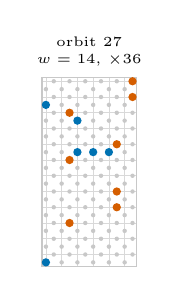
\begin{tikzpicture}[scale=0.2]
  \torus
  \node[Lq, minimum size=3pt] at \LposT{0}{0} {};
  \node[Lq, minimum size=3pt] at \LposT{0}{10} {};
  \node[Lq, minimum size=3pt] at \LposT{2}{7} {};
  \node[Lq, minimum size=3pt] at \LposT{2}{9} {};
  \node[Lq, minimum size=3pt] at \LposT{3}{7} {};
  \node[Lq, minimum size=3pt] at \LposT{4}{7} {};
  \node[Rq, minimum size=3pt] at \RposT{0}{2} {};
  \node[Rq, minimum size=3pt] at \RposT{0}{3} {};
  \node[Rq, minimum size=3pt] at \RposT{0}{6} {};
  \node[Rq, minimum size=3pt] at \RposT{1}{9} {};
  \node[Rq, minimum size=3pt] at \RposT{1}{10} {};
  \node[Rq, minimum size=3pt] at \RposT{3}{1} {};
  \node[Rq, minimum size=3pt] at \RposT{3}{5} {};
  \node[Rq, minimum size=3pt] at \RposT{3}{8} {};
  \node[font=\tiny, align=center] at (2.75,13.4) {orbit 27\\ $w=14$, $\times36$};
\end{tikzpicture}\hfill
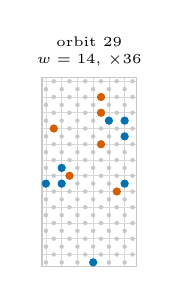
\begin{tikzpicture}[scale=0.2]
  \torus
  \node[Lq, minimum size=3pt] at \LposT{0}{5} {};
  \node[Lq, minimum size=3pt] at \LposT{1}{5} {};
  \node[Lq, minimum size=3pt] at \LposT{1}{6} {};
  \node[Lq, minimum size=3pt] at \LposT{3}{0} {};
  \node[Lq, minimum size=3pt] at \LposT{4}{9} {};
  \node[Lq, minimum size=3pt] at \LposT{5}{5} {};
  \node[Lq, minimum size=3pt] at \LposT{5}{8} {};
  \node[Lq, minimum size=3pt] at \LposT{5}{9} {};
  \node[Rq, minimum size=3pt] at \RposT{0}{3} {};
  \node[Rq, minimum size=3pt] at \RposT{2}{7} {};
  \node[Rq, minimum size=3pt] at \RposT{3}{4} {};
  \node[Rq, minimum size=3pt] at \RposT{5}{6} {};
  \node[Rq, minimum size=3pt] at \RposT{5}{8} {};
  \node[Rq, minimum size=3pt] at \RposT{5}{9} {};
  \node[font=\tiny, align=center] at (2.75,13.4) {orbit 29\\ $w=14$, $\times36$};
\end{tikzpicture}

\caption{Lowest-weight logical X errors found, one panel per orbit (title: orbit id, weight $w$,
number of cosets $\times N$ in the orbit). Top row: all orbits of weight 12; bottom row: nine of
weight 14. Blue: flipped $L$ qubits, orange: flipped $R$ qubits; same layout as \cref{fig:full}
($x$ right, $y$ up). An orbit with fewer than 72 cosets is a pattern that some shift maps to
the same coset (like $y^6$ in \cref{fig:orbit}).}
\label{fig:found}
\end{figure}

%======================================================================
\section{Checking a representative found by any method}

\begin{enumerate}
\item $H_Z e = 0$: it is invisible;
\item $L_Z e = s \ne 0$: it is a logical error, in the claimed coset;
\item its weight $|e|$.
\end{enumerate}
\textbf{Minimality for free at weight 12.} Since the distance is $d = 12$, every non-trivial
invisible error has weight $\ge 12$. So \emph{any} weight-12 representative, however it was
found, is automatically the lightest in its coset. For heavier ones a proof needs the integer
program (or another lower bound).

\section*{Status (2026-10-08)}
\begin{center}
\begin{tabular}{rrrrl}
\toprule
orbit & smallest coset & cosets in orbit & weight & certified by \\
\midrule
0 & 1  & 36 & 12 & distance bound (and MILP) \\
2 & 7  & 9  & 12 & distance bound (and MILP) \\
5 & 64 & 36 & 12 & distance bound; single-block ($L$ and $R$), \cref{fig:logical} \\
1 & 3  & 12 & 14 & MILP, proved optimal \\
\bottomrule
\end{tabular}
\end{center}
Information-set sampling adds 6 more orbits of weight 12, 25 of weight 14 and 60 of weight 16
(\cref{fig:found}); data in \texttt{results/cosets/144\_12\_12\_ldpc/enum\_catalogue.csv}.

\end{document}
